\subsubsection{Sprint goal}
L'obiettivo dello sprint è stato quello di concludere l'epica riguardante la visualizzazione e l'analisi dei tweet.\\
Nello specifico, sono state implementate le seguenti funzionalità:
\begin{itemize}
    \item Ricerca di tweet per intervallo temporale (richiesto dal cliente allo sprint review precedente)
    \item Ricerca di un determinato numero di tweet con una singola ricerca (richiesto dal cliente allo sprint review precedente)
    \item Ricerca di tweet per parola chiave
    \item Mappa per visualizzare la posizione dei tweet con geolocalizzazione
    \item Raccolta di tweet in tempo reale
\end{itemize}


\subsubsection{Backlog}
\userstory%
{Come utente interessato a vedere tweet,\\voglio scegliere un numero di tweet da poter caricare in una volta\\per poterli analizzare in modo aggregato.}%
{5\\(3 frontend + 2 backend)}%
{Possibilità di ricercare un largo numero di tweet scrivendone la quantità in un textbox.\\
Tale quantità serve per la ricerca iniziale e anche per mostrare pagine successive. 
È possibile inoltre ricercare un numero di tweet inizialmente per poi cambiare quantità e cercare una pagina successiva 
(esempio: ricerca di 150 tweet iniziali, poi viene modificata la quantità (dallo stesso textbox) in 20 e si preme su “Pagina successiva”. Il numero di tweet così mostrato diventa 170).}%
{Verificare che il numero di tweet raccolto corrisponda con quello richiesto.}
{Raccolta e analisi di tweet}

\userstory%
{Come utente interessato a vedere tweet,\\voglio scegliere un intervallo di tempo in cui raccogliere tweet\\per analizzarne le tendenze storiche.}%
{5\\(3 frontend + 2 backend)}%
{Possibilità di ricercare dei tweet dato un intervallo temporale. Non deve essere possibile cercare tweet nel futuro.\\
Non deve essere possibile cliccare su “Prossima pagina” quando non ci sono più tweet da visualizzare.}%
{Verificare che i tweet raccolti siano compresi nell'intervallo temporale.}
{Raccolta e analisi di tweet}

\userstory%
{Come utente interessato a vedere tweet,\\voglio poter cercare dei tweet per parola chiave\\per vedere cosa ne pensa la gente a riguardo.}%
{4\\(2 frontend + 2 backend)}%
{Possibilità di cercare tweet per parola o frase chiave. I grafici già presenti devono funzionare anche con questa ricerca.}%
{Richiamare l'API implementata, verificare che il formato sia corretto e che il contenuti dei tweet contenga la parola chiave ricercata.}
{Raccolta e analisi di tweet}

\userstory%
{Come utente interessato ai tweet,\\voglio poter visualizzare su una mappa la posizione dei tweet cercati\\per avere un'idea della località dalla quale sono stati pubblicati.}%
{7\\(3 frontend + 4 backend)}%
{Possibilità di visualizzare una mappa con le posizioni dei tweet ricercati.\\
Se sono presenti più tweet nella stessa zona è possibile aggregarli (in base alla distanza) e mostrare un unico valore, 
ovvero il numero di tweet in tale zona. La mappa deve essere sempre visibile anche durante lo scorrimento della pagina (come i grafici).}%
{Manualmente verificare che la mappa contenga i marker quando sono presenti tweet con geolocalizzazione.}
{Raccolta e analisi di tweet}

\userstory%
{Come utente,\\voglio vedere la posizione di tutti i tweet di una data persona\\per conoscere i suoi spostamenti.}%
{5\\(5 frontend + 0 backend)}%
{Possibilità di inserire il nome utente di una persona e visualizzare su una mappa le posizioni dei suoi tweet e i suoi spostamenti.\\
Per gli spostamenti si mostrano sulla mappa delle frecce basandosi sulla posizione e sulla data del tweet.}%
{Manualmente verificare che la mappa contenga i marker quando sono presenti tweet con geolocalizzazione.}
{Raccolta e analisi di tweet}

\userstory%
{Come lettore di tweet,\\voglio poter vedere i tweet che ricerco in tempo reale\\per sapere cosa la gente posta.}%
{10\\(3 frontend + 7 backend)}%
{Poter scrivere una ricerca e, al click di un pulsante “Live”, vedere tutti i tweet pubblicati in tempo reale a partire da quel momento.}%
{Verificare che il socket implementato restituisca i tweet ricercati, quando disponibili.}
{Raccolta e analisi di tweet}

\newpage
\subsubsection{Esito sprint}
Lo sprint è terminato con la conclusione di tutte le user stories pianificate.\\
Il lavoro si è svolto in linea con l'andamento ideale dei punti. 
Si è osservato una leggera sovrastima delle user stories che ha portato alla conclusione anticipata (di un giorno) dello sprint.\\
\begin{figure}[H]
    \centering
    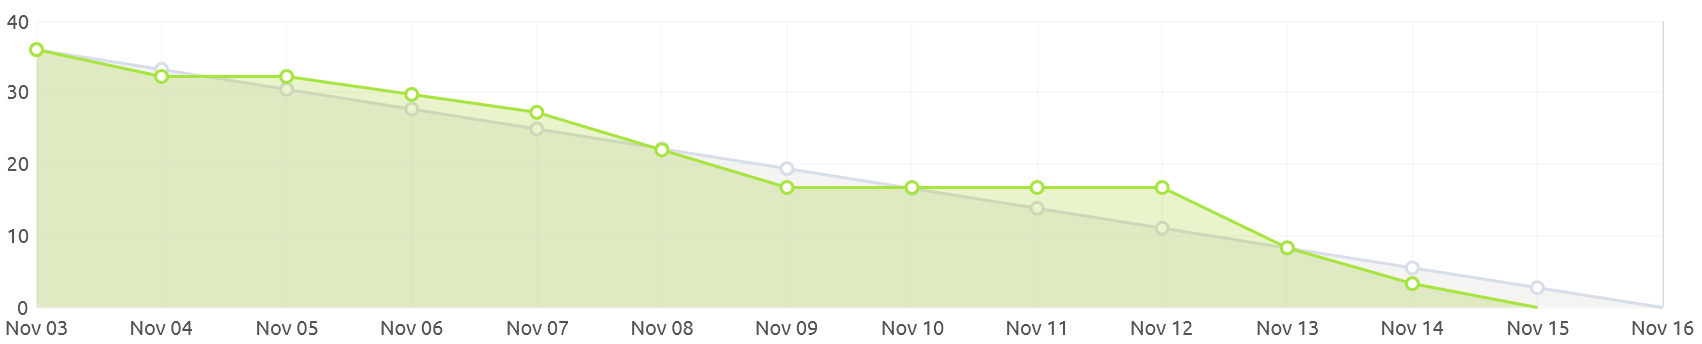
\includegraphics[width=15cm]{./img/sprint2/burndown.png}
    \caption{Burndown sprint 2}
\end{figure}
Le ore di lavoro rispettano il monte ore e sono state distribute principalmente in due periodi di maggiore produttività.
\begin{figure}[H]
    \centering
    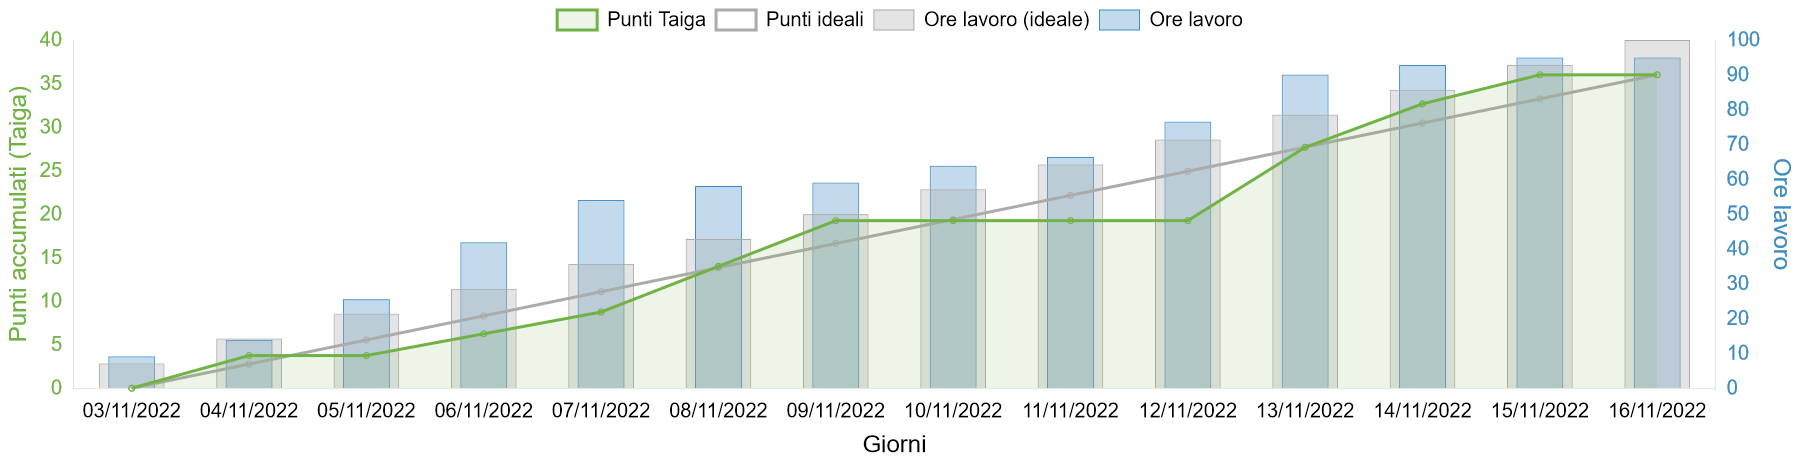
\includegraphics[width=15cm]{./img/sprint2/worktime.png}
    \caption{Progresso dei punti (asse a sinistra) e ore di lavoro (asse a destra)}
\end{figure}


\subsubsection{Sprint review}
Alla sprint review non sono emerse nuove richieste da parte del cliente.


\newpage
\subsubsection{Retrospettiva}
\subsubsection*{Pre-retrospettiva}
Alla pre-retrospettiva effettuata a metà sprint, sono emerse le seguenti problematiche:
\begin{itemize}
    \item Mancanza di test adeguati per il frontend
    \item Le user stories sono state sovrastimate
\end{itemize}
\begin{figure}[H]
    \centering
    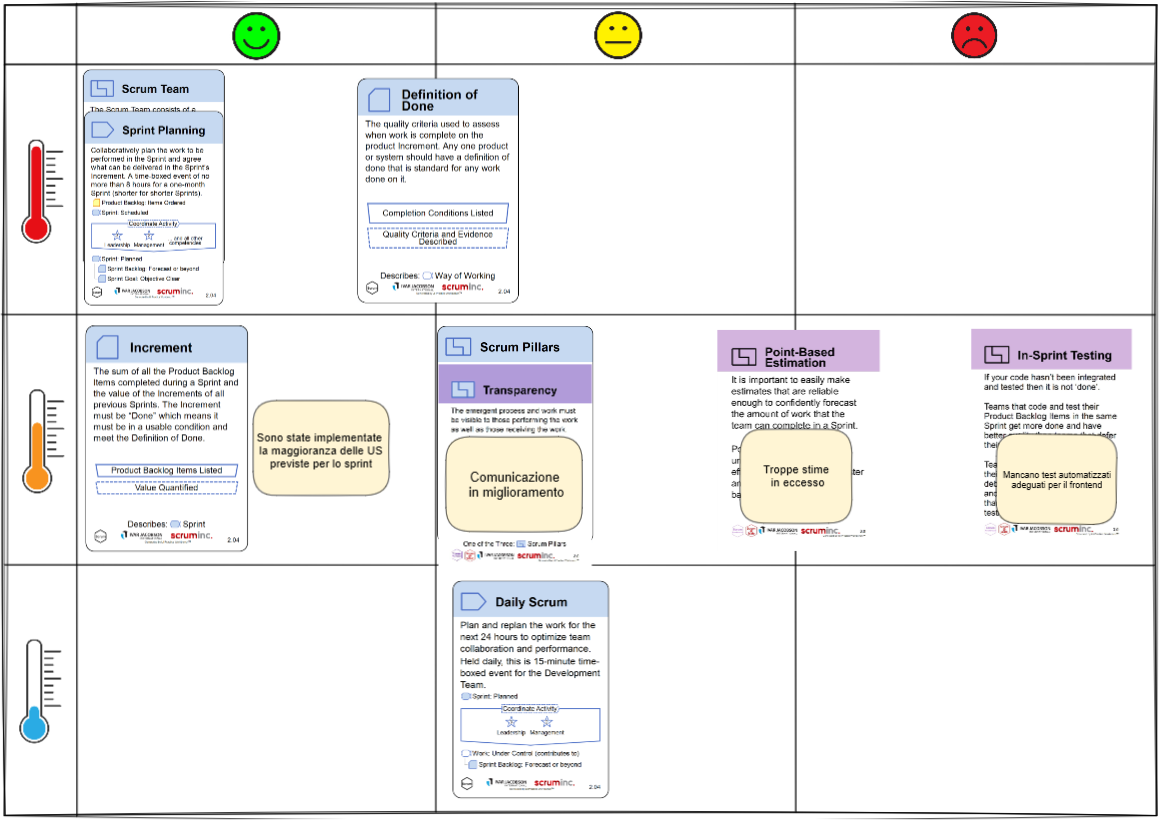
\includegraphics[width=15cm]{./img/sprint2/preretrospettiva.png}
    \caption{Pre-retrospettiva del 10/11/2022}
\end{figure}

\subsection*{Retrospettiva}
Alla retrospettiva di fine sprint sono state confermate le problematiche della pre-retrospettiva.